\documentclass{article}

\input{~/projects/latex/dist/full.tex}
\setLang{de}

\setup{Theoretische Informatik}

\newcommand{\hdelta}{\hat{\delta}}
\newcommand{\qacc}{q_{\text{accept}}}
\newcommand{\qrej}{q_{\text{reject}}}
\newcommand{\ldiag}{L_{\text{diag}}}
\newcommand{\lempty}{L_{\text{empty}}}
\renewcommand{\tc}{\text{Time}}
\newcommand{\spc}{\text{Space}}
\usetikzlibrary{automata, positioning, arrows.meta}

\begin{document}
\startDocument
\usetcolorboxes

\vspace{1cm}
\begin{center}
    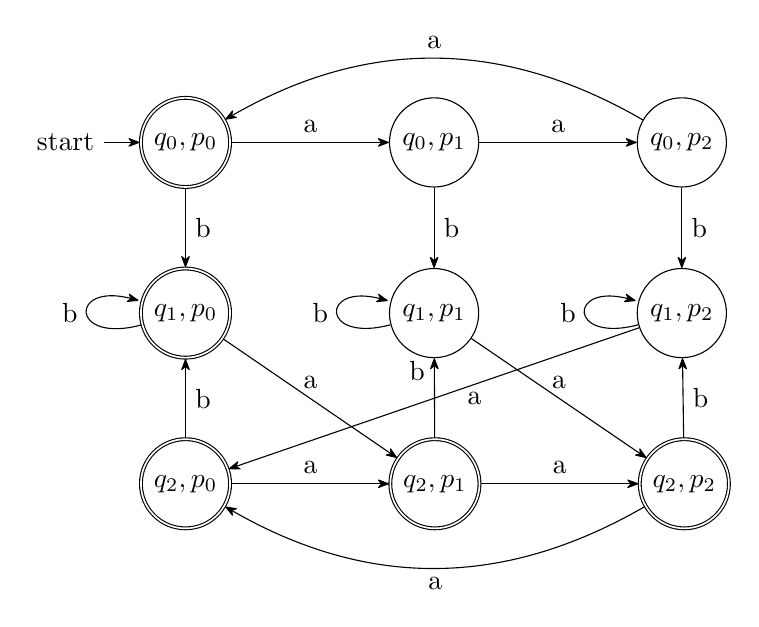
\begin{tikzpicture}[node distance = 1cm and 2cm, >={Stealth[round]}]
        \node[state, initial left, accepting] (q0p0) {$q_0, p_0$};
        \node[state] (q0p1) [right=of q0p0] {$q_0, p_1$};
        \node[state] (q0p2) [right=of q0p1] {$q_0, p_2$};
        \node[state, accepting] (q1p0) [below=of q0p0] {$q_1, p_0$};
        \node[state] (q1p1) [right=of q1p0] {$q_1, p_1$};
        \node[state] (q1p2) [right=of q1p1] {$q_1, p_2$};
        \node[state, accepting] (q2p0) [below=of q1p0] {$q_2, p_0$};
        \node[state, accepting] (q2p1) [right=of q2p0] {$q_2, p_1$};
        \node[state, accepting] (q2p2) [right=of q2p1] {$q_2, p_2$};

        \path[->]
        % Level 0
        (q0p0) edge node [above] {a} (q0p1)
        (q0p1) edge node [above] {a} (q0p2)
        (q0p2) edge [bend right] node [above] {a} (q0p0)
        % Level 0 to level 1
        (q0p0) edge node [right] {b} (q1p0)
        (q0p1) edge node [right] {b} (q1p1)
        (q0p2) edge node [right] {b} (q1p2)
        % Level 1 to level 2
        (q1p0) edge node [above] {a} (q2p1)
        (q1p1) edge node [above] {a} (q2p2)
        (q1p2) edge node [right, xshift=0.3cm] {a} (q2p0)
        % Level 2 to level 1
        (q2p0) edge node [right] {b} (q1p0)
        (q2p1) edge node [above left, yshift=0.1cm] {b} (q1p1)
        (q2p2) edge node [right] {b} (q1p2)
        % Level 2
        (q2p0) edge node [above] {a} (q2p1)
        (q2p1) edge node [above] {a} (q2p2)
        (q2p2) edge [bend left] node [below] {a} (q2p0)
        % ────────────────────────────────────────────────────────────────────
        % Loops on level 1
        (q1p0) edge [loop left] node {b} ()
        (q1p1) edge [loop left] node {b} ()
        (q1p2) edge [loop left] node {b} ();
    \end{tikzpicture}
\end{center}

\vspace{3cm}
\begin{center}
    \begin{Large}
        ``\textit{Sie können also alle C Programme in Kanonischer Ordnung aufzählen. Sollten Sie dies tun? Wahrscheinlich nicht. Was aber zählt ist, sie \textbf{können} es tun}''
    \end{Large}

    \hspace{3cm} - Prof. Dr. Dennis Komm, 2025
\end{center}

\vspace{3cm}
\begin{center}
    HS2025, ETHZ\\[0.2cm]
    \begin{Large}
        Summary of the book \color{MidnightBlue}\fbox{\href{https://link.springer.com/book/10.1007/978-3-658-06433-4}{Theoretische Informatik}}\color{black}
    \end{Large}\\[0.2cm]
    by Prof. Dr. Juraj Hromkovic
\end{center}

\newpage

\printtoc{Orange}

\begin{scriptsize}
    \begin{itemize}
        \item \textit{Note: Definitions, Lemmas, etc are often 1:1 copies from the book or paraphrased (as I did not find an easier way of stating them)}
        \item \textit{Note: In case I forgot to add the PDF page numbers, the PDF page number is given by $P_{\text{PDF}} = P_{\text{Book}} + 15$}
    \end{itemize}
\end{scriptsize}

\newpage


% Combinatorics
\newsection
\section{Combinatorics}
\label{sec:combinatorics}
\subsection{Introduction}
Combinatorics was developed from the willingness of humans to gamble and the fact that everybody wanted to win as much money as possible.

\subsection{Simple counting operations}
The easiest way to find the best chance of winning is to write down all possible outcomes. This can be very tedious though when the list gets longer.

We can note this all down as a list or as a tree diagram. So-called Venn Diagrams might also help represent the relationship between two sets or events. Essentially a Venn Diagram is a graphical representation of set operations such as $A \cup B$.


\subsection{Basic rules of counting}
\subsubsection{Multiplication rule}
If one has $n$ possibilities for a first choice and $m$ possibilities for a second choice, then there are a total of $n \cdot m$ possible combinations.

When we think about a task, and we have an \textbf{and} in between e.g. properties, we need to multiply all the options.

\subsubsection{Addition rule}
If two events are mutually exclusive, the first has $n$ possibilities and the second one has $m$ possibilities, then both events together have $n+m$ possibilities.

When we think about a task, and we have an \textbf{or} in between e.g. properties, then we need to add all the options.


\newpage
\subsection{Factorial}
\begin{definition}[]{Factorial}
    The factorial stands for the product of the first $n$ natural numbers where $n \ge 1$. Notation: $!$
    \[
        n! = n \cdot (n - 1) \cdot (n - 2) \cdot \ldots \cdot 3 \cdot 2 \cdot 1
    \]
    Additionally, $0! = 1$. We read $n!$ as ``\textit{n factorial}''
\end{definition}

\subsubsection{Operations}
We can rewrite $n!$ as $n \cdot (n - 1)!$ or $n \cdot (n - 1) \cdot (n - 2)!$ and so on.

It is also possible to write $7 \cdot 6 \cdot 5$ with factorial notation: $\displaystyle \frac{7!}{4!}$, or in other words, for any excerpt of a factorial sequence: \[n \cdot (n - 1) \cdot \ldots \cdot m = \frac{n!}{(m - 1)!}\]


\subsection{Permutations}
\begin{definition}[]{Permutations}
    A permutation of a group is any possible arrangement of the group's elements in a particular order\\

    \textbf{Permutation rule without repetition:} The number of $n$ \textbf{\textit{distinguishable}} elements is defined as: $n!$
\end{definition}


\subsubsection{Permutation with repetition}
For $n$ elements $n_1,n_2,\ldots,n_k$ of which some are identical, the number of permutations can be calculated as follows:
\[
    p = \frac{n!}{n_1! \cdot n_2! \cdot \ldots \cdot n_k!}
\]
where $n_k$ is the number of times a certain element occurs. 
As a matter of fact, this rule also applies to permutations without repetition, as each element occurs only once, which means the denominator is $1$, hence $\displaystyle \frac{n!}{(1!)^n} = n!$

\inlineex \smallhspace CANADA has $6$ letters, of which $3$ letters are the same. So the word consists of $3$ A's, which can be arranged in $3!$ different ways, a C, N and D, which can be arranged in $1!$ ways each. Therefore, we have:
\[
    \frac{6!}{3!\cdot 1! \cdot 1! \cdot 1!} = \frac{6!}{3!} = 6 \cdot 5 \cdot 4 = 120
\]

Since $1!$ equals $1$, we can always ignore all elements that occur only once, as they won't influence the final result.


\newpage
\subsection{Variations}
\begin{definition}[]{Variations}
    A \textbf{\textit{variation}} is a selection of $k$ elements from a universal set that consists of $n$ \textit{distinguishable} elements.\\

    \textbf{Variation rule without repetition:} The $_n\mbox{P}_k$ function is used to \textit{\textbf{place}} $n$ elements on $k$ places. In a more mathematical definition:
    The number of different variations consisting of $k$ different elements selected from $n$ distinguishable elements can be calculated as follows:

    \[
        \frac{n!}{(n - k)!} = _n\mbox{P}_k
    \]
\end{definition}

\subsubsection{Variations with repetition}
If an element can be selected more than once and the order matters, the number of different variations consisting of $k$ elements selected from $n$ distinguishable elements can be calculated using $n^k$



\subsection{Combinations}
\begin{definition}[]{Combination}
    A combination is a selection of $k$ elements from $n$ elements in total without any regard to order or arrangement.

    \textbf{Combination rule without repetition:} \[
        _n\mbox{C}_k = {n\choose k} = \frac{_n\mbox{P}_k}{k!} = \frac{n!}{(n - k)! \cdot k!}
    \]
\end{definition}

\subsubsection{Combination with repetition}
In general the question to ask for combinations is, in how many ways can I distribute $k$ objects among $n$ elements?
\[
    _{n + k - 1}\mbox{C}_k = {n + k - 1\choose k} = \frac{(n + k - 1)!}{k!(n - 1)!}
\]



\subsection{Binomial Expansion}
\label{sec:binomial-expansion}
Binomial expansion is usually quite hard, but it can be much easier than it first seems. The first term of the expression of $(a + b)^n$ is always $1 a^n b^0$. Using the formula for combination without repetition, we can find the coefficients of each element:

\begin{center}
    \includegraphics[width=0.6\linewidth]{./assets/binomialExpansion.png}
\end{center}

This theory is based on the Pascal's Triangle and the numbers of row $n$ correspond to the coefficients of each element of the expanded term.

We can calculate the coefficient of each part of the expanded term $k$ with combinatorics as follows: $\displaystyle {n\choose k}$

\begin{formula}[]{Binomial Expansion}
    \textbf{\textit{\underbar{In general:}}}
    \[
        (a + b)^n = 1a^nb^0 + {n\choose 1} a^{n-1}b^{1} + {n\choose 2} a^{n-2}b^{2} + \ldots + {n\choose n - 1} a^{1}b^{n - 1} + {n\choose n} a^{0}b^{n}
    \]
\end{formula}


\subsection{Overview}
\includegraphics[width=1\linewidth]{./assets/overview.png}



% ┌                                                ┐
% │                   Alphabets                    │
% └                                                ┘
\newsection
\section{Alphabete, Wörter, Sprachen und Darstellung von Problemen}
\stepcounter{subsection}
\input{parts/01_languages-problems/00_alphabet.tex}
\input{parts/01_languages-problems/01_algorithmic-problems.tex}
\input{parts/01_languages-problems/02_kolmogorov-complexity.tex}


% ────────────────────────────────────────────────────────────────────
% ┌                                                ┐
% │                    Automata                    │
% └                                                ┘
\newsection
\section{Endliche Automaten}
\stepcounter{subsection}
\subsection{Darstellung}
Folgende Fragen müssen zur Definition eines Berechnungsmodells beantwortet werden:
\begin{enumerate}
    \item Welche elementaren Operationen stehen zur Verfügung (um das Programm zusammenzustellen)?
    \item Wie funktioniert der Speicher?
    \item Wie funktioniert die Eingabe (und welches Alphabet verwendet sie)?
    \item Wie funktioniert die Ausgabe (und welches Alphabet verwendet sie)?
\end{enumerate}
Endliche Automaten haben keinen Speicher, mit Ausnahme des Zeigers (can be understood similarly to a program counter)

Ein endlicher Automat mit dem Eingabealphabet $\Sigma = \{ a_1, \ldots, a_k \}$ darf nur den Operationstyp \texttt{select} verwenden.
\begin{align*}
    \texttt{select } input & = a_1 \texttt{ goto } i_1 \\[-0.2cm]
    \vdots                                             \\
    input                  & = a_k \texttt{ goto } i_k
\end{align*}
Alternativ, falls $|\Sigma| = 2$ (typischerweise für $\alphabets{bool}$), kann man statt \texttt{select} auch \texttt{if\dots then\dots else} nutzen.
Typischerweise werden solche Programme für Entscheidungsprobleme genutzt und die Checks sind dann:
\begin{align*}
    \texttt{if } input = 1 \texttt{ then goto } i \texttt{ else goto } j
\end{align*}
Wir wählen eine Teilmenge $F \subseteq \{ 0, \ldots, m - 1 \}$, wobei $m$ die Anzahl Zeilen des Programms ist.
Ist die Zeile auf der das Programm endet ein Element von $F$, so akzeptiert das Programm die Eingabe.
Die Menge $F$ wird auch die \bi{vom Programm akzeptierte Sprache} genannt
%
Ein Programm $A$ arbeitet dann Buchstabe für Buchstabe das Eingabewort ab und springt so also kontinuierlich durch das Programm bis die Eingabe endet.
Mit formaleren Begriffen ist das Eingabewort als \bi{Band} dargestellt, welches von einem \bi{Lesekopf}, der sich nur nach links oder rechts bewegen kann gelesen wird und die gelesene Eingabe dann dem \bi{Programm} weitergibt.

Diese Notation wird jedoch heute kaum mehr verwendet (because \texttt{goto} bad, Prof. Roscoe would approve).
Heute verwendet man meist einen gerichteten Graphen $G(A)$:
\begin{itemize}
    \item Hat so viele Knoten (= \bi{Zustände}) wie das Programm $A$ Zeilen hat
    \item Wenn das Programm beim Lesen von Symbol $b$ von Zeile $i$ auf $j$ sprint, so gibt es in $G(A)$ eine gerichtete Kante $(i, j)$ von Knoten $i$ nach Knoten $j$ mit Markierung $b$. Sie wird als \bi{Übergangsfunktion} bezeichnet
    \item Jeder Knoten hat den Ausgangsgrad $|\Sigma|$ (wir müssen alle Fälle abdecken)
\end{itemize}

% TODO: Clean up (make it look less crowded)
\begin{definition}[]{Endlicher Automat}
    Ist eine Quitupel $M = (Q, \Sigma, \delta, q_0, F)$:
    \begin{enumerate}[label=\textit{(\roman*)}]
        \item $Q$ ist eine endliche Menge von \bi{Zuständen}
        \item $\Sigma$ ist das \bi{Eingabealphabet}
        \item $\delta: Q \times \Sigma \rightarrow Q$ ist die \bi{Übergangsfunktion}. $\delta(q, a) = p$ bedeutet Übergang von Zustand $q$ nach $p$ falls in $q$ $a$ gelesen wurde
        \item $q_0 \in Q$ ist der \bi{Anfangszustand}
        \item $F \subseteq Q$ ist die \bi{Menge der akzeptierenden Zustände}
    \end{enumerate}
    \rmvspace
    \rmvspace
    \begin{multicols}{2}
        \begin{itemize}
            \item \bi{Konfiguration}: Element aus $Q \times \Sigma^*$
            \item \bi{Startkonfiguration} auf $x$: $(q_0, x)$
            \item \bi{Endkonfiguration}: Jede aus $Q \times \{ \lambda \}$
        \end{itemize}
    \end{multicols}
    \rmvspace
    \rmvspace
    \begin{itemize}
        \item \bi{Schritt}: Relation auf Konfigurationen $\bigvdash{M}{} \subseteq (Q \times \Sigma^*) \times (Q \times \Sigma^*$ definiert durch $(q, w) \bigvdash{M}{} (p, x) \Leftrightarrow w = ax, a \in \Sigma \text{ und } \delta(q, a) = p$. Einfacher: Anwendung von $\delta$ auf die aktuelle Konfiguration
        \item \bi{Berechnung} $C$: Endliche Folge von Konfigurationen, $C_i \bigvdash{M}{} C_{i + 1}$.
              Auf Eingabe $x \in \Sigma^*$, $C_0$ Startkonfiguration und $C_n$ Endkonfiguration.
              Falls $C_n \in F \times \{ \lambda \}$, $C$ \bi{akzeptierende Berechnung}, $M$ \bi{akzeptiert Wort} $x$.
              Anderenfalls ist $C$ eine \bi{verwerfende Berechnung} und $M$ \bi{verwirft (akzeptiert nicht) das Wort} $x$
        \item \bi{Akzeptierte Sprache} $L(M) = \{ w \in \Sigma^* \divides \text{$M$ akzeptiert das Wort } w \text{ und $M$ endet in Endkonfig.} \}$
        \item $\mathcal{L}_{EA} = \{ L(M) | M \text{ ist ein EA}\}$ ist die Klasse aller Sprachen die von endlichen Automaten akzeptiert werden, auch genannt \bi{Klasse der regulären Sprachen} und für jede Sprache $L \in \mathcal{L}_{EA}$ gilt: $L$ regulär
    \end{itemize}
\end{definition}
Die Übergangsfunktion kann auch gut graphisch oder tabellarisch (wie eine Truth-Table) dargestellt werden.

$M$ ist in der Konfiguration $(q, w) \in Q \times \word$, wenn $M$ in Zustand $q$ ist und noch das Suffix $w$ zu lesen hat (also auf dem Eingabeband hinter dem Zeiger noch $w$ steht)

\begin{definition}[]{Reflexive und transitive Hülle}
    Sei $M = (Q, \Sigma, \delta, q_0, F)$ ein endlicher Automat. Die reflexive und transitive Hülle $\bigvdash{M}{*}$ der Schrittrelation $\bigvdash{M}{}$ von $M$ als
    $(q, w) \bigvdash{M}{*} (p, u) \Leftrightarrow (q = p \land w = u) \lor \exists k \in \N - \{ 0 \}$ so dass
    \begin{enumerate}[label=\textit{(\roman*)}]
        \item $w = a_1\ldots a_ku, a_i \in \Sigma$ für $i = 1, \ldots, k$
        \item $\exists r_1, \ldots, r_{k - 1} \in Q$, so dass
              $(q, w) \bigvdash{M}{} (r_1, a_2 \ldots a_k u) \bigvdash{M}{} (r_2, a_3 \ldots a_k u) \bigvdash{M}{} \ldots (r_{k - 1}, a_k u) \bigvdash{M}{} (p, u)$
    \end{enumerate}
    Wir definieren $\hat{\delta}: Q \times \Sigma^* \rightarrow Q$ durch
    \rmvspace
    \rmvspace
    \begin{multicols}{2}
        \begin{enumerate}[label=\textit{(\roman*)}]
            \item $\hat{\delta}(q, \lambda) = q \smallhspace \forall q \in Q$
            \item $\hat{\delta}(q, wa) = \delta(\hat{\delta}(q, w), a) \forall a \in \Sigma, w \in \Sigma^*, q \in Q$
        \end{enumerate}
    \end{multicols}
\end{definition}

\begin{intuition}[]{$\bigvdash{M}{*}$ und $\hdelta(q, w)$}
    $(q, w) \bigvdash{M}{*} (p, u)$ bedeutet, dass es eine Berechnung von $M$ gibt, die von der Konfiguration $(q, w)$ zu $(p, u)$ führt.
    Eine wichtiger Aspekt ist die Transitivität, was ja dann bedeutet, dass es (beliebig viele) Zwischenschritte gibt, so dass die Relation erfüllt ist.
    Oder noch viel einfacher: Es gibt irgendwieviele Zwischenschritte zwischen dem linken und rechten Zustand

    $\hdelta(q, w) = p$ repräsentiert den letzen Zustand der Berechnung ausgehend von $(q, w)$.
    Etwas formaler bedeutet dies $(q, w) \bigvdash{M}{*} (p, \lambda)$, also falls $M$ im Zustand $q$ das Wort $w$ zu lesen beginnt, $M$ im Zustand $p$ endet.
\end{intuition}
Also gilt $L(M) = \{ w \in \Sigma^* \divides (q_0, w) \bigvdash{M}{*} (p, \lambda) \smallhspace \forall p \in F \} = \{ w \in \Sigma^* \divides \hdelta(q_0, w) \in F \}$.

Das folgende Lemma bezieht sich auf den Automaten $M$, den wir in der Tabelle weiter unten definieren.
Der Automat entscheidet, ob die beiden Zahlen gerade oder ungerade sind.
Dies kann man aber auch folgendermassen in formaler Ausdrucksweise ausdrücken:

\inlinelemma $L(M) = \{ w \in \{ 0, 1 \}^* \divides |w|_0 + |w|_1 \equiv 0 \text{ mod } 2 \}$

Jeder EA teilt die Menge $\Sigma^*$ in $|Q|$ Klassen
$\class[p] = \{ w \in \Sigma^* \divides \hdelta(q_0, w) = p \} = \{ w \in \Sigma^* \divides (q_0, w) \bigvdash{M}{*} (p, \lambda) \}$ auf
und entsprechend gilt:
\begin{align*}
    \bigcup_{p \in Q} \class[p] = \Sigma^* \text{ und } \class[p] \cup \class[q] = \emptyset \smallhspace \forall p \neq q \in Q
\end{align*}

In dieser Terminologie gilt dann $L(M) = \bigcup_{p \in F} \class[p]$.
Die Notation $|w|_i$ bedeutet die Länge der Buchstaben $i$ in $w$.

Wir können $L(M)$ mit Klassen bestimmen und haben eine Äquivalenzrelation $x R_\delta y \Leftrightarrow \hat{\delta}(q_0, x) = \hat{\delta}(q_0, y)$ auf $\Sigma^*$.
Man beweist die Korrektheit der gewählten Klassen oft mithilfe von Induktion über die Länge der Wörter.
Wir beginnen mit der Länge an Wörtern der Länge kleiner gleich zwei und erhöhen dies dann während unseres Induktionsschrittes.

\inlineintuition Die Klassen sind Mengen, die hier Wörter mit gewissen Eigenschaften, die der EA bestimmt hat, wenn er in Zustand $q_i$ endet, enthalten.
Diese Eigenschaften sind beispielsweise, dass alle Wörter, für die der EA in Zustand $q_i$ endet mit einer gewissen Sequenz enden, sie einen gewissen Zahlenwert haben, etc.

Die Klassen bestimmen wir vor dem Beginn der Induktion auf und jede Klasse repräsentiert einen der Zustände.
\begin{wrapfigure}[5]{l}{0.3\textwidth}
    \begin{tables}{ccc}{Zustand & 0     & 1}
              $q_0$         & $q_2$ & $q_1$ \\
              $q_1$         & $q_3$ & $q_0$ \\
              $q_2$         & $q_0$ & $q_3$ \\
              $q_3$         & $q_1$ & $q_2$ \\
    \end{tables}
\end{wrapfigure}
Haben wir einen EA $M$ mit nebenstehender Tabelle, so sind die Klassen $\class[q_0], \ldots, \class[q_3]$, definiert durch:
\rmvspace
\begin{align*}
    \class[q_0] & = \{ w \in \wordbool \divides |w|_0 \text{ und } |w|_1 \text{ sind gerade} \}          \\
    \class[q_1] & = \{ w \in \wordbool \divides |w|_0 \text{ ist gerade, } |w|_1 \text{ ist ungerade} \} \\
    \class[q_2] & = \{ w \in \wordbool \divides |w|_0 \text{ ist ungerade, } |w|_1 \text{ ist gerade} \} \\
    \class[q_3] & = \{ w \in \wordbool \divides |w|_0 \text{ und } |w|_1 \text{ sind ungerade} \}
\end{align*}
%
Falls ein EA $A$ genügend anschaulich und strukturiert dargestellt ist, kann man die Sprache $L(A)$ auch ohne Beweis bestimmen.

Idealerweise konstruieren wir einen EA so, dass wir die Menge aller Wörter aus $\Sigma^*$ so in Klassen aufteilen,
sodass Wörter mit denselben Eigenschaften in derselben Klasse liegen und wir dann Übergangsfunktionen zu anderen Klassen finden,
die nur einen Buchstaben aus $\Sigma$ zum Wort hinzufügen

\inlineex Das Buch enthält einige zwei gute Beispiele (Beispiel 3.1 und 3.2) mit ausführlichen Erklärungen ab Seite 58 (= Seite 73 im PDF).

% Starting P63 = P78
\newpage
\subsection{Simulationen}
Der Begriff der Simulation ist nicht ein formalisiert, da er je nach Fachgebiet, eine etwas andere Definition hat.
Die engste Definition fordert, dass jeder elementare Schritt der zu Berechnung, welche simuliert wird, durch eine Berechnung in der Simulation nachgemacht wird.
Eine etwas schwächere Forderung legt fest, dass in der Simulation auch mehrere Schritte verwendet werden dürfen.

Es gibt auch eine allgemeinere Definition, die besagt, dass nur das gleiche Eingabe-Ausgabe-Verhalten gilt und der Weg, oder die Berechnungen, welche die Simulation geht, respektive durchführt, wird ignoriert, respektive wird nicht durch die Definition beschränkt.

\textit{Hier werden wir aber die enge Definition verwenden}

\inlinelemma Wir haben zwei EA $M_1 = (Q_1, \Sigma, \delta_1, q_{01}, F_1)$ und $M_2 = (Q_2, \Sigma, \delta_2, q_{02}, F_2)$, die auf dem Alphabet $\Sigma$ operieren.
Für jede Mengenoperation $\odot \in \{ \cup, \cap, - \}$ existiert ein EA $M$, so dass $L(M) = L(M_1) \odot L(M_2)$

Was dieses Lemma nun aussagt ist folgendes: Man kann einen endlichen Automaten bauen, so dass das Verhalten von zwei anderen EA im Bezug auf die Mengenoperation simuliert wird.
Ein guter, ausführlicher Beweis dieses Lemmas findet sich im Buch auf Seite 64 (= Seite 79 im PDF)

Dieses Lemma hat weitreichende Nutzen. Besonders ist es also möglich einen modularen EA zu bauen, in dem Teile davon in kleinere und einfachere EA auszulagern, die dann wiederverwendet werden können.

\stepcounter{examples}
\inlineex Dieses Beispiel im Buch ist sehr gut erklärt und findet sich auf Seiten 65, 66 \& 67 (= Seite 80, 81 \& 82 im PDF)

\subsection{Beweise der Nichtexistenz}
Im Gegensatz zum Beweis, dass eine bestimmte Klasse von Programmen (Algorithmen) ein Problem lösen kann
(was ein einfacher Existenzbeweis ist, bei welchem man eine korrekte Implementation liefern kann),
ist der Beweis, dass diese Klasse von Programmen (Algorithmen) dies nicht tun kann viel schwieriger,
da man (logischerweise) nicht für alle (undendlich vielen) Programme zeigen kann, dass sie das Problem nicht lösen.

In diesem Kurs werden wir aber vorerst nur die Klasse der endlichen Automaten behandlen, welche sehr stark eingeschränkt sind,
was diese Beweise verhältnismässig einfach macht.
Falls also ein EA $A$ für zwei unterschiedliche Wörter $x$ und $y$ im gleichen Zustand endet (also $\hdelta(q_0, x) = \hdelta(q_0, y))$),
so heisst das für uns von jetzt an, dass $A$ nicht zwischen $x$ und $y$ unterscheiden kann:

\begin{lemma}[]{Unterscheidung von Wörtern}
    Sei $A$ ein EA über $\Sigma$ und $x \neq y \in \Sigma^*$ so dass
    \begin{align*}
        (q_0, x) \bigvdash{A}{*} (p, \lambda) \text{ und } (q_0, y) \bigvdash{A}{*} (p, \lambda)
    \end{align*}
    für ein $p \in Q$ (also $\hdelta_A (q_0, x) = \hdelta(q_0, y) = p(x, y \in \class [p])$).
    Dann existiert für jedes $z \in \Sigma^*$ ein $r \in Q$, so dass $xz, yz \in \class[p]$, also gilt insbesondere
    \begin{align*}
        xz \in L(A) \Longleftrightarrow yz \in L(A)
    \end{align*}
\end{lemma}

\newsection
\subsection{Nichtdeterminismus}
Einfach gesagt werden hier Automaten behandelt, die zufällige (genannt \bi{nichtdeterministische}) Entscheidungen treffen.
Beispielsweise für ein Entscheidungsproblem $(\Sigma, L)$ bedeutet dies, dass ein nichtdeterministischer EA $A$ eine Sprache $L$ akzeptiert,
falls für jedes $x \in L$ mindestens eine akzeptierende Berechnung von $A$ auf $x$ existiert und für $y \in \word - L$ keine solve existiert.

Wir notieren das Ganze in graphischer Darstellung so, dass wir aus einem Zustand mehrere Übergänge mit dem gleichen Eingabesymbol erlauben.

\begin{definition}[]{nichtdeterministischer Endlicher Automat (NEA)}
    Ein NEA ist eine Quitupel $M = (Q, \Sigma, \delta, q_0, F)$:
    \begin{enumerate}[label=\textit{(\roman*)}]
        \item \bi{Zustandsmenge:} $Q$ ist eine endliche Menge
        \item \bi{Eingabealphabet:} $\Sigma$ ist ein Alphabet
        \item \bi{Übergangsfunktion:} $\delta : Q \times \Sigma \rightarrow \mathcal{P}(Q)$. $\mathcal{P}(Q)$ ist das Powerset hierbei
        \item \bi{Anfangszustand:} $q_0 \in Q$
        \item \bi{Akzeptierende Zustände:} $F \subseteq Q$
    \end{enumerate}
    Der Rest der Eigenschaften ist sehr ähnlich wie die des deterministischen EA, mit der bedeutenden Ausnahme,
    dass ein Schritt in der $\delta$-Notation nicht $\delta(q, a) = p$, sondern $p \in \delta(q, a)$ ist, da die Übergangsfunktion ja jetzt ins
    Powerset von $Q$ anstelle von nach $Q$ direkt mapped. Die komplette Definition des Schritts ist also:
    \begin{align*}
        (q, w) \bigvdash{M}{} (p, x) \Longleftrightarrow w = ax \text{ für ein } a \in \Sigma \text{ und } p \in \delta(q, a)
    \end{align*}

    Für die $\hdelta$-Funktion, gilt nun $\hdelta(q, \lambda) = \{ q \}$ für jedes $q \in Q$ und wir definieren:
    \begin{align*}
        \hdelta(q, wa) & = \{ p \in Q \divides \text{es existiert ein } r \in \hdelta(q, w), \text{ so dass } p \in \delta(r, a) \} \\
                       & = \bigcup_{r \in \hdelta(q, w)} \delta(r, a) \smallhspace \forall q \in Q, a \in \Sigma, w \in \word
    \end{align*}
    % Page 92 in PDF currently
\end{definition}


\newsection
\section{Turing-Maschinen}
\setcounter{subsection}{2}
\newsection
\subsection{Trigonometrische Interpolation}
\subsubsection{Von Approximation zur Interpolation}
Wir erinnern uns daran, dass wir die Fourier-Approximation durch den Abbruch der unendlichen Fourier-Reihe erhalten, oder in anderen Worten, wir verkleinern die Limiten der Summe.

\fancyremark{DFT mit $N = 2n$ Koeffizienten an Punkten $\frac{l}{N}$ für $l = 0, 1, \ldots, N - 1$}

Der Shift ist hier gegeben durch (für $k \geq 0$ ist $\gamma_k = \hat{f}_N(k)$ und für $k < 0$ ist $\gamma_k = \hat{f}_N(N + k)$)
\begin{align*}
    f_{N - 1}(x)                 & = \sum_{k = -n}^{n - 1} \gamma_k e^{2 \pi ikx} = \sum_{k = 0}^{n - 1} \gamma_k e^{2\pi ikx} + \sum_{k = -n}^{-1} \gamma_k e^{2\pi ikx} \\
    \Leftrightarrow f_{N - 1}(x) & = \frac{1}{N} \left( \sum_{j = 0}^{N - 1} \left( f\left( \frac{j}{n} \right)
        \sum_{k = -n}^{n - 1} e^{2\pi ik \left( x - \frac{j}{N} \right)} \right) \right)
\end{align*}

\vspace{-1pc}

Wenn wir die Funktion nun an der Stelle $\frac{l}{N}$ auswerten so erhalten wir:
\rmvspace
\begin{align*}
    f_{N - 1}\left( \frac{l}{N} \right) = \ldots = f\left( \frac{l}{N} \right)
\end{align*}

\vspace{-1.8pc}
was aufgrund der Orthogonalität der diskreten Fourier-Vektoren funktioniert, welche besagt, dass $\displaystyle \sum_{k = -n}^{n - 1} \omega_N^{k(j - l)} = 0$, für alle $j \neq l$.
Für $j = l$ ergibt die Summe $N$.

Dies heisst also, dass die Fourier-Approximation die Interpolationsbedingungen an den Punkten $\frac{l}{N}$ erfüllt,
also können wir die Lösung der Interpolationsaufgabe $p_{N - 1} \left( \frac{l}{N} \right) = f\left( \frac{l}{N} \right)$ f $l = 0, 1, \ldots, N - 1$ im Raum
\rmvspace
\begin{align*}
    \mathcal{T}_N = \text{span}\{ e^{2\pi ijt} \divides j = - \floor{\frac{N - 1}{2}}, \ldots, \floor{\frac{N}{2}} \}
\end{align*}

\rmvspace\rmvspace
folgendermassen finden können: 
\begin{enumerate}[label=(\arabic*)]
    \item Mittels Gleichungssystem $\sum_{j} \gamma_j e^{2\pi ijt_l} = f(t_l)$ für $l = 0, \ldots, N - 1$. Operationen: $\tco{N^3}$
    \item Mittels FFT in $\tco{N \log(N)}$ Operationen, aber nur falls die Punkte äquidistant sind, also $t_l = \frac{l}{N}$.
        Dann ist die Matrix des obigen Gleichungssystems $F^{-1}_N$
\end{enumerate}

\vspace{0.2cm}

Unten findet sich Python code der mit den unterschiedlichen Methoden die Koeffizienten des Trigonometrischen Polynoms bestimmt.
\rmvspace
\begin{code}{python}
    def get_coeff_trig_poly(t: np.ndarray, y: np.ndarray):
    N = y.shape[0]
    if N % 2 == 1:
    n = (N - 1.0) / 2.0
    M = np.exp(2 * np.pi * 1j * np.outer(t, np.arange(-n, n + 1)))
    else:
    n = N / 2.0
    M = np.exp(2 * np.pi * 1j * np.outer(t, np.arange(-n, n)))
    c = np.linalg.solve(M, y)
    return c

    N = 2**12
    t = np.linspace(0, 1, N, endpoint=False)
    y = np.random.rand(N)
    direct = get_coeff_trig_poly(t, y)
    using_fft = np.fft.fftshift(np.fft.fft(y) / N)
    using_ifft = np.conj(np.fft.fftshift(np.fft.ifft(y)))
\end{code}

\newsection
\subsection{Mehrband-Turingmaschinen und Church'sche These}
Die Turingmaschinen sind das Standardmodell der Berechenbarkeitstheorie, aber benötigen einige Modifikationen, um wirklich geeignet zu sein 
(da das Von-Neumann Modell physisch unterschiedliche CPU, Eingabemedium und Speicher für Programme und Daten fordert, aber die TM ein gemeinsames Eingabemedium und Speicher hat).

Eine $k$-Ban-Turingmaschine (für $k \in \N_0$) hat folgende Komponenten:
\begin{itemize}
    \item 
\end{itemize}

\newpage
\subsection{Nichtdeterministische Turingmaschinen}
Die Ideen sind hier sehr ähnlich wie der Übergang zwischen deterministischen und nichtdeterministischen Endlichen Automaten.

\begin{definition}[]{Nichtdeterministische Turingmaschine (NTM)}
    \begin{scriptsize}
        Hier werden nur die wichtigsten Unterschiede aufgezeigt. Formale Definition auf Seiten 113ff. (= Seiten 127ff im PDF) im Buch.
    \end{scriptsize}

    Die Übergangsfunktion geht wieder in die Potenzmenge, also gilt:
    \rmvspace
    \begin{align*}
        \delta : (Q - \{ \qacc, \qrej \}) \times \Gamma \rightarrow \mathcal{P}(Q \times \Gamma \times \{ L, R, N \})
    \end{align*}

    \rmvspace
    und $\delta(p, \cent) \subseteq (\{ (q, \cent, X) \divides q \in Q, X \in \{R, N\} \})$\\

    Die von der NTM $M$ akzeptierte Sprache ist:
    \rmvspace
    \begin{align*}
        L(M) = \{ w \in \word \divides q_0\cent w \bigvdash{M}{*}y\qacc z \text{ für irgendwelche } y, z \in \Gamma^* \}
    \end{align*}
\end{definition}
Ein gutes Beispiel für eine NTM findet sich auf Seiten 114ff. im Buch (= Seite 128ff. im PDF)


\begin{definition}[]{Berechnungsbaum}
    Ein Berechnungsbaum $T_{M, x}$ von $M$ (eine NTM) auf $x$ (Wort aus Eingabealphabet von $M$) ist ein (potentiell un)gerichteter Baum mit einer Wurzel:
    \begin{enumerate}[label=\textit{(\roman*)}]
        \item Jeder Knoten von $T_{M, x}$ ist mit einer Konfiguration beschriftet
        \item Die Wurzel ist der einzige Knoten mit $\deg_{\text{in}}(v) = 0$, ist die Startkonfiguration $q_0\cent x$
        \item Jeder mit $C$ beschriftete Knoten hat genauso viele Kinder wie $C$ Nachfolgekonfigurationen hat und die Kinder sind mit diesen Nachfolgekonfigurationen markiert.
    \end{enumerate}
\end{definition}
Diese Bäume können natürlich auch für nichtdeterministischen MTM verwendet werden.

Im Vergleich zu den Berechnungsbäumen von NEA sind die Bäume von NTM nicht immer endlich.

\inlinetheorem Sei $M$ eine NTM. Dann existiert eine TM $A$, so dass $L(M) = L(A)$ 
und falls $M$ keine unendlichen Berechnungen auf Wörtern aus $(L(M))^C$ hat, dann hält $A$ immer.

\inlineproof Auf Seite 117 im Buch (= 131 im PDF). Die Idee zur Umwandlung von $M$ in die TM $A$ ist, dass $A$ Breitensuche im Berechnungsbaum von $M$ durchführt.


\newsection
\section{Berechenbarkeit}
\stepcounter{subsection}
\newsection
\subsection{Trigonometrische Interpolation}
\subsubsection{Von Approximation zur Interpolation}
Wir erinnern uns daran, dass wir die Fourier-Approximation durch den Abbruch der unendlichen Fourier-Reihe erhalten, oder in anderen Worten, wir verkleinern die Limiten der Summe.

\fancyremark{DFT mit $N = 2n$ Koeffizienten an Punkten $\frac{l}{N}$ für $l = 0, 1, \ldots, N - 1$}

Der Shift ist hier gegeben durch (für $k \geq 0$ ist $\gamma_k = \hat{f}_N(k)$ und für $k < 0$ ist $\gamma_k = \hat{f}_N(N + k)$)
\begin{align*}
    f_{N - 1}(x)                 & = \sum_{k = -n}^{n - 1} \gamma_k e^{2 \pi ikx} = \sum_{k = 0}^{n - 1} \gamma_k e^{2\pi ikx} + \sum_{k = -n}^{-1} \gamma_k e^{2\pi ikx} \\
    \Leftrightarrow f_{N - 1}(x) & = \frac{1}{N} \left( \sum_{j = 0}^{N - 1} \left( f\left( \frac{j}{n} \right)
        \sum_{k = -n}^{n - 1} e^{2\pi ik \left( x - \frac{j}{N} \right)} \right) \right)
\end{align*}

\vspace{-1pc}

Wenn wir die Funktion nun an der Stelle $\frac{l}{N}$ auswerten so erhalten wir:
\rmvspace
\begin{align*}
    f_{N - 1}\left( \frac{l}{N} \right) = \ldots = f\left( \frac{l}{N} \right)
\end{align*}

\vspace{-1.8pc}
was aufgrund der Orthogonalität der diskreten Fourier-Vektoren funktioniert, welche besagt, dass $\displaystyle \sum_{k = -n}^{n - 1} \omega_N^{k(j - l)} = 0$, für alle $j \neq l$.
Für $j = l$ ergibt die Summe $N$.

Dies heisst also, dass die Fourier-Approximation die Interpolationsbedingungen an den Punkten $\frac{l}{N}$ erfüllt,
also können wir die Lösung der Interpolationsaufgabe $p_{N - 1} \left( \frac{l}{N} \right) = f\left( \frac{l}{N} \right)$ f $l = 0, 1, \ldots, N - 1$ im Raum
\rmvspace
\begin{align*}
    \mathcal{T}_N = \text{span}\{ e^{2\pi ijt} \divides j = - \floor{\frac{N - 1}{2}}, \ldots, \floor{\frac{N}{2}} \}
\end{align*}

\rmvspace\rmvspace
folgendermassen finden können: 
\begin{enumerate}[label=(\arabic*)]
    \item Mittels Gleichungssystem $\sum_{j} \gamma_j e^{2\pi ijt_l} = f(t_l)$ für $l = 0, \ldots, N - 1$. Operationen: $\tco{N^3}$
    \item Mittels FFT in $\tco{N \log(N)}$ Operationen, aber nur falls die Punkte äquidistant sind, also $t_l = \frac{l}{N}$.
        Dann ist die Matrix des obigen Gleichungssystems $F^{-1}_N$
\end{enumerate}

\vspace{0.2cm}

Unten findet sich Python code der mit den unterschiedlichen Methoden die Koeffizienten des Trigonometrischen Polynoms bestimmt.
\rmvspace
\begin{code}{python}
    def get_coeff_trig_poly(t: np.ndarray, y: np.ndarray):
    N = y.shape[0]
    if N % 2 == 1:
    n = (N - 1.0) / 2.0
    M = np.exp(2 * np.pi * 1j * np.outer(t, np.arange(-n, n + 1)))
    else:
    n = N / 2.0
    M = np.exp(2 * np.pi * 1j * np.outer(t, np.arange(-n, n)))
    c = np.linalg.solve(M, y)
    return c

    N = 2**12
    t = np.linspace(0, 1, N, endpoint=False)
    y = np.random.rand(N)
    direct = get_coeff_trig_poly(t, y)
    using_fft = np.fft.fftshift(np.fft.fft(y) / N)
    using_ifft = np.conj(np.fft.fftshift(np.fft.ifft(y)))
\end{code}

\newpage
\subsection{Die Methode der Reduktion}
% TODO: Add guide for reducing languages
\fancydef{Rekursiv reduzierbare Sprache} Eine Sprache $L_1 \subseteq \word_1$ ist auf $L_2 \subseteq \word_2$ rekursiv reduzierbar, geschrieben $L_1 \leq_R L_2$,
falls $L_2 \in \cL_R \Rightarrow L_1 \in \cL_R$.

\shade{teal}{Intuition:} $L_2$ ist bezüglich der algorithmischen Lösbarkeit mindestens so schwer wie $L_1$. $\cL_R$ ist die Menge aller rekursiv reduzierbaren Sprachen.
Ist also $L_2$ lösbar, so muss auch $L_1$ lösbar sein.

\fancydef{EE-reduzierbare Sprache} $L_1$ ist auf $L_2$ \bi{EE-reduzierbar}, geschrieben $L_1 \leq_{EE} L_2$, wenn eine TM $M$ existiert,
die eine Abbildung $f_M : \word_1 \rightarrow \word_2$ mit der Eigenschaft $x \in L_1 \Leftrightarrow f_M(x) \in L_2$ für alle $x \in \word_1$ berechnet.
Anders ausgedrückt: die TM $M$ reduziert die Sprache $L_1$ auf die Sprache $L_2$

\inlinelemma Falls $L_1 \leq_{EE} L_2$, dann auch $L_1 \leq_R L_2$. \inlineproof Im Buch auf Seite 135 (= 148 im PDF)

Wir müssen also nur zeigen, dass $L_1 \leq_{EE} L_2$ um zu zeigen, dass $L_1 \leq_R L_2$

\inlinelemma Für jede Sprache $L \subseteq \word$ gilt: $L \leq_R L^C$ und $L^C \leq_R L$

\inlinecorollary $(L_\text{diag})^C \notin \cL_R$
\inlineproof Folgt davon, dass $L_\text{diag} \notin \cL_{RE}$ (was heisst, dass $L_\text{diag} \notin \cL_R$)
und nach Lemma 5.4 $L_\text{diag} \leq_R (L_\text{diag})^C$ und das umgekehrte gelten muss.

\inlinelemma $(\ldiag)^C \in \cL_{RE}$
\inlineproof Auf Seite 137 (= 150 im PDF) wird eine Turingmaschine aufgezeigt, die $(L_\text{diag})^C$ akzeptiert.

\inlinecorollary $(\ldiag)^C \in \cL_{RE} - \cL_R$ und daher $\cL_R \subsetneq \cL_{RE}$

Folgende Sprachen sind nicht rekursiv, liegen aber in $\cL_{RE}$

\fancydef{Universelle Sprache} $L_U = \{ \text{Kod}(M)\# w \divides w \in \wordbool \text{ und TM } M \text{ akzeptiert } w \}$

\fancytheorem{Universelle TM} Eine TM $U$, so dass $L(U) = L_U$, also gilt $L_U \in \cL_{RE}$\\
%
\inlineproof Auf Seite 138 (= 151 im PDF)

Was dies bedeutet, es existiert eine TM ohne Haltegarantie, die eine beliebige Turingmaschine auf einer gegebenen Eingabe simulieren kann.
Untenstehendes Resultat bedeutet, dass man das Resultat der Berechnung einer TM $M$ auf einer Eingabe $x$ anders berechnen kann, als die Berechnung von $M$ auf $x$ zu simulieren.

\inlinetheorem $L_U \notin \cL_R$

Wenn jetzt aber $M$ unendlich lange auf $x$ arbeitet, so wissen wir nicht, ob wir die Simulation beenden können. Dies führt zum Halteproblem

\begin{definition}[]{Halteproblem}
    Das Halteproblem ist das Entscheidungsproblem $(\{ 0, 1, \# \}, L_H)$ mit
    \begin{align*}
        L_H = \{ \text{Kod}(M)\# x \divides x \in \{ 0, 1 \}^* \text{ und } M \text{ hält auf } x \}
    \end{align*}
\end{definition}

Dies scheint vorerst nicht ein allzu grosses Problem zu sein, jedoch besagt das nächste Resultat, dass es keinen Algorithmus gibt,
der testen kann, ob ein gegebenes Programm immer terminiert.

\inlinetheorem $L_H \in \cL_R$
\inlineproof Auf Seiten 140 - 142 (153 - 155 im PDF)

Betrachten wir die Sprache $\lempty = \{ \text{Kod}(M) \divides L(M) = \emptyset \}$, die die Kodierungen aller Turingmaschinen enthält,
die die leere Menge (kein Wort) akzeptieren. Es gilt
\rmvspace
\begin{align*}
    (\lempty)^C = \{ x \in \wordbool \divides x \notin \text{Kod}(\overline{M}) \forall \text{ TM } \overline{M} \text{ oder } x = \text{Kod}(M) \text{ und } L(M) \neq \emptyset \}
\end{align*}

\drmvspace
\inlinelemma $(\lempty)^C \in \cL_{RE}$
\inlineproof Auf Seiten 142 - 143 (155 - 156 im PDF)

\inlinelemma $(\lempty)^C \notin \cL_R$

Wir haben als wiederum die Nichtexistenz eines Algorithmus zur Überprüfung, ob ein gegebenes Programm die leere Menge akzeptiert.
Ein Beweis dazu findet sich auf Seiten 143 und 144 im Buch (156 - 157 im PDF)

\inlinecorollary $\lempty \notin \cL_R$

\inlinecorollary $L_{EQ} = \{ \text{Kod}(M)\# \text{Kod}(\overline{M}) \divides L(M) = L(\overline{M}) \}$ ist nicht entscheidbar (also $L_{EQ} \notin \cL_R$)

\subsection{Der Satz von Rice}
\inlinedef $L$ heisst \bi{semantisch nichttriviales Entscheidungsproblem über Turingmaschinen}, falls folgende Bedingungen gelten:
\begin{enumerate}[label=(\roman*)]
    \item Es gibt eine TM $M_1$, so dass $\text{Kod}(M_1) \in L$ (also $L \neq \emptyset$)
    \item Es gibt eine TM $M_2$, so dass $\text{Kod}(M_2) \notin L$ (also sind nicht alle Kodierungen in $L$)
    \item für zwei TM $A$ und $B$: $L(A) = L(B) \Rightarrow \text{Kod}(A) \in L \Leftrightarrow \text{Kod}(B) \in L$
\end{enumerate}

Sei $L_{H, \lambda} = \{ \text{Kod}(M) \divides M \text{ hält auf } \lambda \}$ ein spezifisches Halteproblem.

\inlinelemma $L_{H, \lambda} \notin \cL_R$
\inlineproof Auf Seite 146 im Buch (= 159 im PDF)

\begin{theorem}[]{Satz von Rice}
    Jedes semantisch nichttriviale Entscheidungsproblem über Turingmaschinen ist unentscheidbar.
\end{theorem}
\inlineproof Ausführlich im Buch auf Seiten 146 - 149 beschrieben (= 159 - 162 im PDF)
\stepcounter{subsection}

\subsection{Die Methode der Kolmogorov-Komplexität}
\inlinetheorem Das Probelem, für jedes $x \in \wordbool$ die Kolmogorov-Komplexität $K(x)$ von $x$ zu berechnen ist algorithmisch unlösbar.

\inlinelemma Falls $L_H \in \cL_R$, dann existiert ein Algorithmus zur Berechnung der Kolmogorov-Komplexität $K(x)$ für jedes $x\in \wordbool$


\newsection
\section{Komplexitätstheorie}
\stepcounter{subsection}
\newsection
\subsection{Trigonometrische Interpolation}
\subsubsection{Von Approximation zur Interpolation}
Wir erinnern uns daran, dass wir die Fourier-Approximation durch den Abbruch der unendlichen Fourier-Reihe erhalten, oder in anderen Worten, wir verkleinern die Limiten der Summe.

\fancyremark{DFT mit $N = 2n$ Koeffizienten an Punkten $\frac{l}{N}$ für $l = 0, 1, \ldots, N - 1$}

Der Shift ist hier gegeben durch (für $k \geq 0$ ist $\gamma_k = \hat{f}_N(k)$ und für $k < 0$ ist $\gamma_k = \hat{f}_N(N + k)$)
\begin{align*}
    f_{N - 1}(x)                 & = \sum_{k = -n}^{n - 1} \gamma_k e^{2 \pi ikx} = \sum_{k = 0}^{n - 1} \gamma_k e^{2\pi ikx} + \sum_{k = -n}^{-1} \gamma_k e^{2\pi ikx} \\
    \Leftrightarrow f_{N - 1}(x) & = \frac{1}{N} \left( \sum_{j = 0}^{N - 1} \left( f\left( \frac{j}{n} \right)
        \sum_{k = -n}^{n - 1} e^{2\pi ik \left( x - \frac{j}{N} \right)} \right) \right)
\end{align*}

\vspace{-1pc}

Wenn wir die Funktion nun an der Stelle $\frac{l}{N}$ auswerten so erhalten wir:
\rmvspace
\begin{align*}
    f_{N - 1}\left( \frac{l}{N} \right) = \ldots = f\left( \frac{l}{N} \right)
\end{align*}

\vspace{-1.8pc}
was aufgrund der Orthogonalität der diskreten Fourier-Vektoren funktioniert, welche besagt, dass $\displaystyle \sum_{k = -n}^{n - 1} \omega_N^{k(j - l)} = 0$, für alle $j \neq l$.
Für $j = l$ ergibt die Summe $N$.

Dies heisst also, dass die Fourier-Approximation die Interpolationsbedingungen an den Punkten $\frac{l}{N}$ erfüllt,
also können wir die Lösung der Interpolationsaufgabe $p_{N - 1} \left( \frac{l}{N} \right) = f\left( \frac{l}{N} \right)$ f $l = 0, 1, \ldots, N - 1$ im Raum
\rmvspace
\begin{align*}
    \mathcal{T}_N = \text{span}\{ e^{2\pi ijt} \divides j = - \floor{\frac{N - 1}{2}}, \ldots, \floor{\frac{N}{2}} \}
\end{align*}

\rmvspace\rmvspace
folgendermassen finden können: 
\begin{enumerate}[label=(\arabic*)]
    \item Mittels Gleichungssystem $\sum_{j} \gamma_j e^{2\pi ijt_l} = f(t_l)$ für $l = 0, \ldots, N - 1$. Operationen: $\tco{N^3}$
    \item Mittels FFT in $\tco{N \log(N)}$ Operationen, aber nur falls die Punkte äquidistant sind, also $t_l = \frac{l}{N}$.
        Dann ist die Matrix des obigen Gleichungssystems $F^{-1}_N$
\end{enumerate}

\vspace{0.2cm}

Unten findet sich Python code der mit den unterschiedlichen Methoden die Koeffizienten des Trigonometrischen Polynoms bestimmt.
\rmvspace
\begin{code}{python}
    def get_coeff_trig_poly(t: np.ndarray, y: np.ndarray):
    N = y.shape[0]
    if N % 2 == 1:
    n = (N - 1.0) / 2.0
    M = np.exp(2 * np.pi * 1j * np.outer(t, np.arange(-n, n + 1)))
    else:
    n = N / 2.0
    M = np.exp(2 * np.pi * 1j * np.outer(t, np.arange(-n, n)))
    c = np.linalg.solve(M, y)
    return c

    N = 2**12
    t = np.linspace(0, 1, N, endpoint=False)
    y = np.random.rand(N)
    direct = get_coeff_trig_poly(t, y)
    using_fft = np.fft.fftshift(np.fft.fft(y) / N)
    using_ifft = np.conj(np.fft.fftshift(np.fft.ifft(y)))
\end{code}

\newpage
\subsection{Komplexitätsklassen und die Klasse P}
\begin{definition}[]{Komplexitätsklasen}
    Für alle Funktionen $f, g : \N \rightarrow \R^+$ definieren wir:
    \begin{align*}
        \text{TIME}(f)  & = \{ L(B) \divides B \text{ ist eine MTM mit } \tc_B(n) \in \tco{f(n)} \}  \\
        \text{SPACE}(g) & = \{ L(A) \divides A \text{ ist eine MTM mit } \spc_A(n) \in \tco{g(n)} \} \\
        \text{DLOG}     & = \text{SPACE}(\log_2(n))                                                  \\
        \text{P}        & = \bigcup_{c \in \N} \text{TIME}(n^c)                                      \\
        \text{PSPACE}   & = \bigcup_{c \in \N} \text{SPACE}(n^c)                                     \\
        \text{EXPTIME}  & = \bigcup_{d \in \N} \text{TIME}(2^{n^d})
    \end{align*}
\end{definition}

\inlinelemma Für alle $t : \N \rightarrow \R^+$ gilt $\text{TIME}(t(n)) \subseteq \text{SPACE}(t(n))$
\inlinecorollary $\text{P} \subseteq \text{PSPACE}$

\begin{definition}[]{Platz- und Zeitkonstruierbarkeit}
    Eine Funktion $t : \N \rightarrow \N$ heisst \bi{platzkonstruierbar}, falls eine $1$-Band-TM $M$ existiert, so dass
    \begin{enumerate}
        \item $\spc_M(n) \leq s(n) \smallhspace \forall n \in \N$
        \item für jede Eingabe $0^n$ für $n \in \N$, generiert $M$ das Wort $0^{s(n)}$ auf ihrem Arbeitsband und hält in $\qacc$
    \end{enumerate}

    \vspace{0.25cm}

    Eine Funktion $s : \N \rightarrow \N$ heisst \bi{zeitkonstruierbar}, falls eine MTM $A$ existiert, so dass
    \begin{enumerate}
        \item $\tc_A(n) \in \tco{t(n)}$
        \item für jede Eingabe $0^n$ für $n \in \N$, generiert $A$ das Wort $0^{t(n)}$ auf dem ersten Arbeitsband und hält in $\qacc$
    \end{enumerate}
\end{definition}
Wichtig ist, dass wir hier nicht \textit{zwingend} eine $1$-Band-TM konstruieren müssen, eine MTM geht auch.

% TODO: Possibly include construction guide here

\inlinelemma Sei $s$ platzkonstruierbar und $M$ eine MTM mit $\spc_M(x) \leq s(|x|) \ \forall x \in L(M)$.
Dann existiert MTM $A$ mit $L(A) = L(M)$ und $\spc_A(n) \leq s(n)$, es gilt also $\spc_A(y) \leq s(|y|) \ \forall y \in \Sigma_M$

\inlinelemma Sei $t$ zeitkonstruierbar und $M$ eine MTM mit $\tc_M(x) \leq t(|x|) \ \forall x \in L(M)$.
Dann existiert eine MTM $A$ mit $L(A) = L(M)$ und $\tc_A(n) \in \tco{t(n)}$

\inlinetheorem Für jede Funktion $s$ mit $s(n) \geq \log_2(n)$ gilt $\text{SPACE}(s(n)) \subseteq \bigcup_{c\in \N} \text{TIME}(c^{s(n)})$

Obiger Satz trifft auch für $s(n)$-platzbeschränkten TM zu, die nicht halten, aber nur, wenn $s(n)$ platzkonstruierbar ist.

\inlinecorollary $\text{DLOG} \subseteq \text{P}$ und $\text{PSPACE} \subseteq \text{EXPTIME}$

Die Korollare \ref{corollary:6-1} und \ref{corollary:6-2} geben zusammen $\text{DLOG} \subseteq \text{P} \subseteq \text{PSPACE} \subseteq \text{EXPTIME}$


\inlinetheorem Für $s_1, s_2 : \N \rightarrow \N$ mit folgenden Eigenschaften:
\drmvspace
\begin{multicols}{3}
    \begin{enumerate}
        \item $s_2(n) \geq \log_2(n)$
        \item $s_2$ ist platzkonstruierbar
        \item $s_1(n) = o(s_2(n))$
    \end{enumerate}
\end{multicols}

\drmvspace\rmvspace
Dann gilt: $\text{SPACE}(s_1) \subsetneq \text{SPACE}(s_2)$


\inlinetheorem Für $t_1, t_2 : \N \rightarrow \N$ mit folgenden Eigenschaften:
\drmvspace
\begin{multicols}{2}
    \begin{enumerate}
        \item $t_2$ ist platzkonstruierbar
        \item $t_1(n) \cdot \log_2(t_1(n)) = o(t_2(n))$
    \end{enumerate}
\end{multicols}

\drmvspace\rmvspace
Dann gilt: $\text{TIME}(s_1) \subsetneq \text{TIME}(s_2)$

In den Sechzigerjahren entstand folgende ``Definition'' von parktisch lösbaren Problemen:
\begin{center}
    \fbox{
        \parbox{16cm}{
            \textit{Ein Problem ist praktisch lösbar genau dann, wenn ein polynomialer Algorithmus zu seiner Lösung existiert.
                Die Klasse P ist die Klasse der praktisch entscheidbaren Probleme}
        }
    }
\end{center}

\newpage
\subsection{Nichtdeterministische Komplexitätsmasse}

\begin{definition}[]{Zeit- und Speicherkomplexität}
    Sei $M$ eine NMTM oder MTM und $x \in L(M) \subseteq \word$. $\tc_M(x)$ ist die länge einer kürzesten akzeptierenden Berechnung von $M$ auf $x$
    und $\tc_M(n) = \max(\{ \tc_M(x) \divides x \in L(M) \text{ und }|x| = n \} \cup \{ 0 \} )$.

    \vspace{0.25cm}

    $\spc_M(C_i)$ ist die Speicherkomplexität von Konfiguration $C_i$ und $\spc_M(C) = \max\{ \spc_M(C_i) \divides i = 1, 2, \ldots, m \}$.
    Zudem ist $\spc_M(x) = \min\{ \spc_M(C) \divides C \text{ ist akzeptierende Berechnung von $M$ auf } x \}$.
    Ausserdem ist $\spc_M(n) = \max(\{ \spc_M(x) \divides x \in L(M) \text{ und } |x| = n \} \cup \{ 0 \})$
\end{definition}


\begin{definition}[]{Komplexitätsklassen}
    Für alle $f, g : \N \rightarrow \R^+$ definieren wir:
    \begin{align*}
        \text{NTIME}(f)  & = \{ L(M) \divides M \text{ ist eine NMTM mit } \tc_M(n) \in \tco{f(n)} \}  \\
        \text{NSPACE}(g) & = \{ L(M) \divides M \text{ ist eine NMTM mit } \spc_M(n) \in \tco{g(n)} \} \\
        \text{NLOG}      & = \text{NSPACE}(\log_2(n))                                                  \\
        \text{NP}        & = \bigcup_{c \in \N} \text{NTIME}(n^c)                                      \\
        \text{NPSPACE}   & = \bigcup_{c \in \N} \text{NSPACE}(n^c)
    \end{align*}
\end{definition}


\inlinelemma Für alle $t$ und $s$ mit $s(n) \geq \log_2(n)$ gilt: $\text{NTIME}(t) \subseteq \text{NSPACE}(t)$, $\text{NSPACE}(s) \subseteq \bigcup_{c \in \N} \text{NTIME}(c^{s(n)})$

\inlinetheorem Für jedes $t : \N \rightarrow \R^+$ und jedes platzkonstruierbare $s$ mit $s(n) \geq \log_2(n)$ gilt:
\rmvspace
\begin{multicols}{2}
    \begin{enumerate}[label=(\roman*)]
        \item $\text{TIME}(t) \subseteq \text{NTIME}(t)$
        \item $\text{SPACE}(t) \subseteq \text{NSPACE}(t)$
        \item $\text{NTIME}(s(n)) \subseteq \text{SPACE}(s(n)) \subseteq \bigcup_{c \in \N} \text{TIME}(c^{s(n)})$
    \end{enumerate}
\end{multicols}

\drmvspace
\inlinecorollary $\text{NP} \subseteq \text{PSPACE}$

\inlinetheorem Für jede platzkonstruierbare Funktion $s$ mit $s(n) \geq \log_2(n)$ gilt
\rmvspace
\begin{align*}
    \text{NSPACE}(s(n)) \subseteq \bigcup_{c \in \N} \text{TIME}(c^{s(n)})
\end{align*}

\drmvspace
\inlinecorollary $\text{NLOG} \subseteq \text{P}$ und $\text{NPSPACE} \subseteq \text{EXPTIME}$


\fancytheorem{Satz von Savitch} Sei $s$ mit $s(n) \geq \log_2(n)$ eine platzkonstruierbare Funktion. Dann gilt:
\rmvspace
\begin{align*}
    \text{NSPACE}(s(n)) \subseteq \text{SPACE}(s(n)^2)
\end{align*}

\drmvspace
\inlinecorollary $\text{PSPACE} = \text{NPSPACE}$

Aus den obigen Resultaten resultiert die Komplexitätsklassenhierarchie der sequentiellen Berechnungen:
\begin{align*}
    \text{DLOG} \subseteq \text{NLOG} \subseteq \text{P} \subseteq \text{NP} \subseteq \text{PSPACE} \subseteq \text{EXPTIME}
\end{align*}

\newpage
\subsection{Die Klasse NP und Beweisverifikation}

\newpage
\subsection{NP-Vollständigkeit}
Es sind mittlerweile über 3000 Probleme bekannt, für welche wir keinen Algorithmus kennen, der in polynomieller Zeit läuft.
Es ist aber bis jetzt niemandem gelungen, eine höhere untere Schranke für alle zu beweisen, als $\tcl{n}$.

Wie bereits bei der Berechenbarkeit benutzen wir eine Reduktion.
Falls jedes Problem aus $NP$ effizient auf ein Problem $L \in NP$ reduzierbar ist, so ist $L$ schwer.

\begin{definition}[]{Polynomielle Reduktion}
    $L_1 \subseteq \word_1$ ist \bi{polynomiell reduzierbar auf} $L_2 \subseteq \word_2$, geschrieben $L_1 \leq_p L_2$,
    falls eine polynomielle TM $A$ existiert, die für jedes Wort $x \in \word_1$ ein Word $A(x) \in \word_2$ berechnet, so dass
    \rmvspace
    \begin{align*}
        x \in L_1 \Longleftrightarrow A(x) \in L_2
    \end{align*}

    \drmvspace
    $A$ wird eine polynomielle Reduktion von $L_1$ auf $L_2$ genannt.
\end{definition}
Wieder bedeutet $L_1 \leq_p L_2$, dass $L_2$ mindestens so schwer ist wie $L_1$

\begin{definition}[]{$NP$-Schwer}
    Eine Sprache $L$ ist \bi{$NP$-Schwer}, falls für alle $L' \in NP$ gilt $L' \leq_p L$.

    Eine Sprache $L$ ist \bi{$NP$-Vollständig}, falls
    \drmvspace
    \begin{multicols}{2}
        \begin{enumerate}[label=\textit{(\roman*)}]
            \item $L \in NP$
            \item $L$ $NP$-Schwer ist.
        \end{enumerate}
    \end{multicols}
\end{definition}

\inlinelemma Falls $L \in P$ und $L$ ist $NP$-schwer, dann gilt $P = NP$

\fancytheorem{Cook} $SAT$ ist $NP$-Vollständig

Der Beweis hierfür liefert eine grobe Struktur für weitere Beweise dieser Art und ist auf Seiten 199 - 205 im Buch (= Seiten 211 - 217 im PDF) zu finden.


\inlinelemma Falls $L_1 \leq_p L_2$ und $L_1$ ist $NP$-Schwer, so ist auch $L_2$ $NP$-Schwer

Betrachten wir folgende 


\newsection
\section{Grammatiken}
\stepcounter{subsection}
\newsection
\subsection{Trigonometrische Interpolation}
\subsubsection{Von Approximation zur Interpolation}
Wir erinnern uns daran, dass wir die Fourier-Approximation durch den Abbruch der unendlichen Fourier-Reihe erhalten, oder in anderen Worten, wir verkleinern die Limiten der Summe.

\fancyremark{DFT mit $N = 2n$ Koeffizienten an Punkten $\frac{l}{N}$ für $l = 0, 1, \ldots, N - 1$}

Der Shift ist hier gegeben durch (für $k \geq 0$ ist $\gamma_k = \hat{f}_N(k)$ und für $k < 0$ ist $\gamma_k = \hat{f}_N(N + k)$)
\begin{align*}
    f_{N - 1}(x)                 & = \sum_{k = -n}^{n - 1} \gamma_k e^{2 \pi ikx} = \sum_{k = 0}^{n - 1} \gamma_k e^{2\pi ikx} + \sum_{k = -n}^{-1} \gamma_k e^{2\pi ikx} \\
    \Leftrightarrow f_{N - 1}(x) & = \frac{1}{N} \left( \sum_{j = 0}^{N - 1} \left( f\left( \frac{j}{n} \right)
        \sum_{k = -n}^{n - 1} e^{2\pi ik \left( x - \frac{j}{N} \right)} \right) \right)
\end{align*}

\vspace{-1pc}

Wenn wir die Funktion nun an der Stelle $\frac{l}{N}$ auswerten so erhalten wir:
\rmvspace
\begin{align*}
    f_{N - 1}\left( \frac{l}{N} \right) = \ldots = f\left( \frac{l}{N} \right)
\end{align*}

\vspace{-1.8pc}
was aufgrund der Orthogonalität der diskreten Fourier-Vektoren funktioniert, welche besagt, dass $\displaystyle \sum_{k = -n}^{n - 1} \omega_N^{k(j - l)} = 0$, für alle $j \neq l$.
Für $j = l$ ergibt die Summe $N$.

Dies heisst also, dass die Fourier-Approximation die Interpolationsbedingungen an den Punkten $\frac{l}{N}$ erfüllt,
also können wir die Lösung der Interpolationsaufgabe $p_{N - 1} \left( \frac{l}{N} \right) = f\left( \frac{l}{N} \right)$ f $l = 0, 1, \ldots, N - 1$ im Raum
\rmvspace
\begin{align*}
    \mathcal{T}_N = \text{span}\{ e^{2\pi ijt} \divides j = - \floor{\frac{N - 1}{2}}, \ldots, \floor{\frac{N}{2}} \}
\end{align*}

\rmvspace\rmvspace
folgendermassen finden können: 
\begin{enumerate}[label=(\arabic*)]
    \item Mittels Gleichungssystem $\sum_{j} \gamma_j e^{2\pi ijt_l} = f(t_l)$ für $l = 0, \ldots, N - 1$. Operationen: $\tco{N^3}$
    \item Mittels FFT in $\tco{N \log(N)}$ Operationen, aber nur falls die Punkte äquidistant sind, also $t_l = \frac{l}{N}$.
        Dann ist die Matrix des obigen Gleichungssystems $F^{-1}_N$
\end{enumerate}

\vspace{0.2cm}

Unten findet sich Python code der mit den unterschiedlichen Methoden die Koeffizienten des Trigonometrischen Polynoms bestimmt.
\rmvspace
\begin{code}{python}
    def get_coeff_trig_poly(t: np.ndarray, y: np.ndarray):
    N = y.shape[0]
    if N % 2 == 1:
    n = (N - 1.0) / 2.0
    M = np.exp(2 * np.pi * 1j * np.outer(t, np.arange(-n, n + 1)))
    else:
    n = N / 2.0
    M = np.exp(2 * np.pi * 1j * np.outer(t, np.arange(-n, n)))
    c = np.linalg.solve(M, y)
    return c

    N = 2**12
    t = np.linspace(0, 1, N, endpoint=False)
    y = np.random.rand(N)
    direct = get_coeff_trig_poly(t, y)
    using_fft = np.fft.fftshift(np.fft.fft(y) / N)
    using_ifft = np.conj(np.fft.fftshift(np.fft.ifft(y)))
\end{code}



\end{document}
